\section{Theoretical Analysis}
\label{sec:theoretical}

\par In this section, the circuit shown in figure \ref{fig:1} is analysed theoretically.
<<<<<<< HEAD
\par The following analysis will be made considering the ideal model of an OP-AMP, where its gain is infinite, with an infinite input impedance and 0 output impedance. Pratically speaking an OP-AMP has diferent values for the properties refered above. This are the most important differences, but of course, aren't the only ones, this differences will be talk about again when we compare the results and will also help explain the differences encountered in Octave and NGspice.  
\par This circuit will behave as a non-inverting amplifier, and since the objective of this lab assignment is to have the least gain and frequency deviation. This circuit also behaves as a band-pass filter and the components responsible for this feature are the capacitors since the lower and higher cut off frequency are calculated from this components like it will be shown below.

\subsection{First Point}

\par Our theoretical analysis starts by computing the gain and the imput and output impedances at central frequency.
\par First we have to calculate the central frequency and for that we'll have to discover the lower and higher cut off frequencies, those will be the poles, discovered using the characteristic equations. The formulae are,

\begin{equation}
	w_{CutOff} = frac{1}{R1C1}
\end{equation}

\begin{equation}
	w_{CutOff} = frac{1}{R2C2}
\end{equation}

, as expected, the higher value will be the higher cut off frequency, $w_H$, and the lower will be the lower cut off frequency, $w_L$. Then to discover the central frequency, $w_0$, we use 

\begin{equation}
	w_{0} = \sqrt(w_L w_H)
\end{equation}

\Par Since we want a central frequency of $f_0 = 1000 Hz$ ($w_0 = 2000\pi rad/s$), and from the previous equations we get the following relation

\begin{equation}
	2000\pi = frac{1}{\sqrt(R1C1R2C2)}
\end{equation}

\par We can now choose the best values for the resistors and capacitors to get the smallest frequency deviation. We found that using a capacitor of 220nF and a parallel of capacitors of 220 for C2 and C1, respectively, and resistors of $1k\Omega$, would get the best results.
=======
\par Like we said in section \ref{sec:introduction}, both of the stages of the amplifier are going to be analysed in a more detailed way in this section.
\par Let's begin with the gain stage. The gain stage consists of a common emitter amplifier, with a NPN transistor, which allows us to obtain a high input impedance ($Z_{i_1}$), and a high gain $A_V$. However, this type of amplifier has a very high output impedance ($Z_{o_1}$), which causes a degeneration of the signal output. In order to solve this problem, the gain stage is connected to an output stage, which consists of a common collector amplifier, whith a PNP transistor. This stage has a gain a little bit lower than 1, but still very close to 1, and a very high input impedance ($Z_{o_2}$), which preserve the high gain of the previous stage. In addition, this circuit has a very low output impedance ($Z_{o_2}$), which means that almost all the gain is going to be delivered to the speaker.

\subsection{First Point}

\par Our theoretical analysis starts by computing the operating point, using the theoretical DC model studied. In order to do this, we harnessed the mesh method provided in the Octave script to which we added the new components.
\par The values of currents are presented in table \ref{tab:currents}, as well as the values of $V_{CE}$ and $V_{BE}$, and $V_{EC}$ and $V_{EB}$, respectively for the NPN and the PNP transistors, in order to prove that they're working in the forward active region ($V_{CE} > V_{BEON}$ and $V_{EC} > V_{EBON}$).

>>>>>>> d0b080297fc0b7e965087175cb535c02ef7a19c1

\vspace{5mm}
\begin{table}[H]
	\centering
	\begin{tabularx}{0.9\textwidth} {
 	    | >{\raggedright\arraybackslash}X
  	    | >{\raggedleft\arraybackslash}X | }
	\hline
<<<<<<< HEAD
	\input{../mat/frequencias_tab.tex}
	\end{tabularx}
	\caption{All frequencies computed [rad/s]}
=======
	Low Cut Off & 9.090909e+03 rad/s\\ \hline
High Cut Off & 4.545455e+03 rad/s\\ \hline
Medio & 6.428243e+03 rad/s\\ \hline
Input Impedance & 1.000000e+03 \\ \hline
Output Impedance & 3.333333e+02 \\ \hline
Gain & 3.366667e+01 \\ \hline
Gain & 3.054400e+01 dB \\ \hline

	\end{tabularx}
	\caption{$V_{CE}$, $V_{BE}$, $V_{EC}$, $V_{EB}$, and circulation current values}
>>>>>>> d0b080297fc0b7e965087175cb535c02ef7a19c1
	\label{tab:currents}
\end{table}
\vspace{5mm}

<<<<<<< HEAD
\par Now since we know the central frequency we can calculate the gain at that frequency knowing the transfer function. We now show the formula used, the explanation of this formula will be made in the next subsection when we deduce the the tranfer function.

\begin{equation}
	Gain = |frac{1}{1 + j R2 C2 w_0} frac{j R1 C1 w_0}{1 + j R1 C1 w_0} (1 + frac{R3}{R4})| 
\end{equation}

\begin{equation}
	Gain dB = 20 log_{10}(Gain)
\end{equation}
=======
\subsection{Second Point}

\par The second point in this analysis consists in computing the gain and input and output impedances separately for each stage.
\par In order to do this kind of analysis we have to consider the incremental model of the circuit.


\par In order to compute the gain of each stage, we used the formulae which were taught in the theoretical classes (which were also given in advance in Octave's script). We can use this simplified formulae, because we are assuming medium/high frequencies. Based on this assumption, we can replace the capacitor with a short circuit.
\par In a similar way, we computed the input and output impedances, using the formulae given in the theoretical classes (which were also given in advance in Octave's script), which are based on the same assumption.
\par To make things a little bit more clear, the input/output impedances are determined by connecting, for example, a voltage source to the stage's input/output and replacing the output/input with a short circuit. By determining the current that flows across the added voltage source, we can determine the input/output impedance by just applying Ohm's law. This values are shown in tables 2 and 3, respectively for the input and the output stages. The overall output impedance and gain are shown in table 4.
>>>>>>> d0b080297fc0b7e965087175cb535c02ef7a19c1

\vspace{5mm}
\begin{table}[H]
	\centering
	\begin{tabularx}{0.9\textwidth} {
 	    | >{\raggedright\arraybackslash}X
  	    | >{\raggedleft\arraybackslash}X | }
	\hline
<<<<<<< HEAD
	\input{../mat/ganhos_tab.tex}
	\end{tabularx}
	\caption{Computed Gains}
	\label{tab:currents}
\end{table}
\vspace{5mm}
 
\par To calculate the input and output impedance we just had to analise the circut and knowing the input and output impedance of the OP-AMP we determine that the input impedance is equal to the impedance of R1 in series with C1 and the output impedance is equal to the impedance of R2 in parallel with C2.

\begin{equation}
	Z_i = R1 + frac{1}{j w_0 C2}
\end{equation}

\begin{equation}
	Z_o = frac{R2}{1 + j w_0 C2 R2}
\end{equation}

\vspace{5mm}
=======
	\input{../mat/ponto2_tab.tex}
	\end{tabularx}
	\caption{Gain, input and output impedances - gain stage}
	\label{tab:stage1}
\end{table}
\vspace{5mm}

>>>>>>> d0b080297fc0b7e965087175cb535c02ef7a19c1
\begin{table}[H]
	\centering
	\begin{tabularx}{0.9\textwidth} {
 	    | >{\raggedright\arraybackslash}X
  	    | >{\raggedleft\arraybackslash}X | }
	\hline
<<<<<<< HEAD
	\input{../mat/impedancias_tab.tex}
	\end{tabularx}
	\caption{Computed impedances [$\Omega$]}
	\label{tab:currents}
\end{table}
\vspace{5mm}

Now lets analise the frequency response of the circuit, and for, we'll deduce the tranfer function of the circuit.
 
\subsection{Second Point}

\par Knowing that it is a non-inverting amplifier we know the following relation

\begin{equation}
	frac{v_6}{v_3} = 1 + frac{R3}{R4}
\end{equation}

, but we still don't have a relation between $v_0$ and $v_I$, to do that we have to relate them with $v_6$ and $v_3$. 
\par Lets find a relation between $v_0$ and $v_6$, applying the voltage divider we have

\begin{equation}
	v_o = frac{frac{1}{jwC2}}{frac{1}{jwC2 + R2}}v_6 = frac{1}{1 + jR2C2w}
\end{equation}

\par Now to find a relation between $v_3$ and $v_I$, we'll also apply the voltage divider, 

\begin{equation}
	v_3 = frac{R1}{frac{1}{jwC1 + R1}}v_I = frac{jwR1C1}{1 + jR1C1w}v_I
\end{equation}

\par Now that we have the relations that we needed and knowing that $s=jw$, we can combine the last three equations to get

\begin{equation}
	frac{v_o}{v_I} = T(s) = frac{1}{1 + R2 C2 s} frac{s R1 C1}{1 + s R1 C1} (1 + frac{R3}{R4})
\end{equation}

\par This was the formula used to get the gain at the central frequency in the previous subsection. Doing $T_{dB}(s) = 20log_{dB}(|T(s)|)$, we can plot for frequencies ranging from 10 Hz to 100MHz. We can see in the following figure this plot in a logarithmic scale.

\begin{figure}[H] 
	\centering
	\includegraphics[width=1\linewidth]{teorica.eps}
	\caption{Frequency response [dB] ($\frac{V_o(f)}{V_I(f)}$)}
\end{figure}

\par To conclude this theoretical analysis we show now the frequency and gain deviation, the cost and the theoretical Merit and we also show the values of the components used.
=======
	\input{../mat/ponto3_tab.tex}
	\end{tabularx}
	\caption{Gain, input and output impedances - output stage}
	\label{tab:stage2}
\end{table}
\vspace{5mm}

\begin{table}[H]
	\centering
	\begin{tabularx}{0.9\textwidth} {
 	    | >{\raggedright\arraybackslash}X
  	    | >{\raggedleft\arraybackslash}X | }
	\hline
	\input{../mat/ponto4_tab.tex}
	\end{tabularx}
	\caption{Overal gain and output impedance}
	\label{tab:overall}
\end{table}
\vspace{5mm}

\par As one might observe, the input impedance of the output stage ($Z_{i_2}$) is substantially greater than the output impedance of the gain stage ($Z_{o_1}$). Hence, because the voltage divider applied at the input of the output stage is given by

\begin{equation}
	v_{i_2}= \frac{Z_{i_2}}{Z_{o_1}+Z_{i_2}} \cdot v_{o_1}
\end{equation}

\noindent if $Z_{o_1}<<Z_{i_2}$, we can say that $v_{i_2} \approx v_{o_1}$. It's worth to mention that the gain of the output stage is approximately 1, so overall there is no significant signal loss when the two stages are put together.

\begin{equation}
	AV2dB = -9.207782e-02 \Rightarrow AV2 = 0.989455 \approx 1
\end{equation}

\subsection{Third Point}

\par The third point of this theoretical analysis is to compute the frequency responce $\frac{V_o(f)}{V_i(f)}$. 
\par In order to do so, we can't neglect the effect of the capacitors, since only this component's impedance is frequency dependent.
\par Being that, we calculated the transfer function of the circuit. To do that we calculated the two poles, the lower and high cut off frequency based on the document provided by the professor. Knowing that we built our transfer function and plotted the following figure.

\begin{figure}[H] 
	\centering
	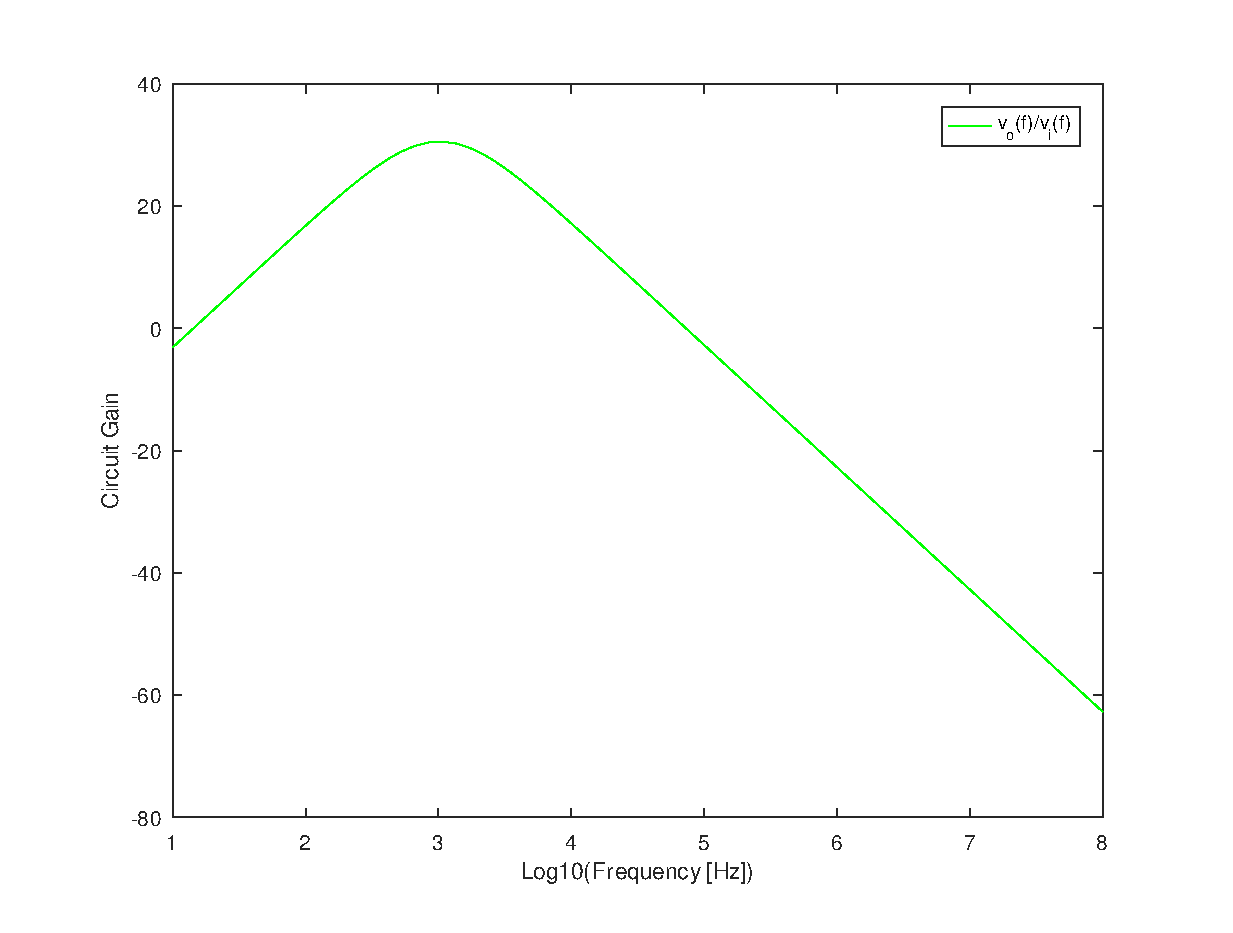
\includegraphics[width=1\linewidth]{teoria.eps}
	\caption{Frequency response of the amplifier ($\frac{V_o(f)}{V_i(f)}$)}
\end{figure}

\par Finally, the theoretical merit is shown below, as well as the high and low cutoff frequencies, the cost and the bandwidth.
>>>>>>> d0b080297fc0b7e965087175cb535c02ef7a19c1

\vspace{5mm}
\begin{table}[H]
	\centering
	\begin{tabularx}{0.9\textwidth} {
 	    | >{\raggedright\arraybackslash}X
  	    | >{\raggedleft\arraybackslash}X | }
	\hline
<<<<<<< HEAD
	\input{../mat/componentes_tab.tex}
	\end{tabularx}
	\caption{Values of the components used ([$\Omega$],[F])}
	\label{tab:currents}
\end{table}
\vspace{5mm}

\vspace{5mm}
\begin{table}[H]
	\centering
	\begin{tabularx}{0.9\textwidth} {
 	    | >{\raggedright\arraybackslash}X
  	    | >{\raggedleft\arraybackslash}X | }
	\hline
	\input{../mat/final_tab.tex}
	\end{tabularx}
	\caption{Frequency and gain deviation, cost and merit}
	\label{tab:currents}
\end{table}
\vspace{5mm}
=======
	\input{../mat/ponto5_tab.tex}
	\end{tabularx}
	\caption{Theoretical variables of merit}
	\label{tab:merit1}
\end{table}
\vspace{5mm}

>>>>>>> d0b080297fc0b7e965087175cb535c02ef7a19c1
